% !TEX root = ../main.tex

O documento de visão tem como objetivo definir uma visão geral do projeto, apresentar os problemas, os requisitos funcionais, não funcionanis, atores, entre outras informações que serão definidos com o cliente a fim de garantir que a equipe de desenvolvimento e o cliente estejam na maior sincronia possível \cite{IBM:2014:Online}.

%-----------------------------------------------------------------------------------------------------------
\subsection{Posicionando}
\subsubsection{Oportunidade de Negócios}

Atualmente, as ferramentas no mercado possuem limitações, como de qualidade, falta de flexibilidade na gerência, ou até mesmo o fechamento do código, que pode ser considerado uma limitação devida a redução de mão de obra para manutenção e evolução.

\subsubsection{Instrução do Problema}

A \er{} possui diversas \textit{rotas} possíveis para se seguir, como, por exemplo a rota ágil, tradicional ou até mesmo uma mistura das duas.

Infelizmente, cada ferramenta de gerência de requisitos é voltada para uma dessas possibilidades, tornando díficil a tarefa voltada para outras, gerando assim nos engenheiros de requisitos a necessidade de aprender a utilizar diversas ferramentas para poder organizar projetos com \textit{rotas} diferentes.

A utilização de apenas uma ferramenta que abrangesse as duas metodologias e ainda uma mistura das duas resolveria todo problema de gerência de requisitos em projetos que não se adequam a uma metodologia específica perfeitamente.

\subsubsection{Instrução de Posição do Produto}

Para os engenheiros de \er, a \nomeferramenta~ representará um avanço nas atividades de gerenciamento, pois os mesmos apenas precisarão aprender as funcionalidades de uma ferramenta, simplificando a mudança entre projetos que tomam rotas distintas.

%-----------------------------------------------------------------------------------------------------------
\subsection{Matriz de rastreabilidade de requisitos}

A matriz de rastreabilidade resume o modo como serão organizados os requisitos do sistema, e a escolhida para o projeto esta ilustrada na figura \ref{img:rastreabilidade}.

\begin{figure}[H]
	\centering
	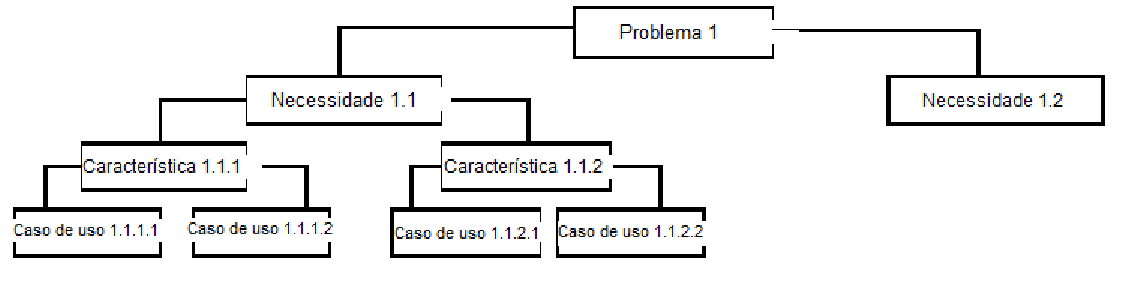
\includegraphics[width=0.8\textwidth]{imgModelagem/diagrama}
	\caption{Matriz de rastreabilidade}
	\label{img:rastreabilidade}
\end{figure}

%-----------------------------------------------------------------------------------------------------------
\subsection{Descrições da Parte Interessada e do Usuário}

Nesta sessão serão identificados e detalhados os interessados e usuários da \nomeferramenta{}.

\subsubsection{Resumo da Parte Interessada e do Usuário}

Para melhor entendimento das características e responsabilidades dos interessados, utilizou-se uma tabela que apresenta todos os interessados no sistema, suas descrições, responsabilidades e os critérios de sucesso de suas funções na equipe, ilustrada na tabela \ref{tab:parteInteressada}. Com esta tabela, pode-se obter o entendimento necessário sobre os interessados e o quão importante eles são para o sucesso do sistema.

\begin{table}[htbp]
\centering
\begin{tabular}{|p{2cm}|p{5cm}|p{4cm}|p{4cm}|}
\hline
%-------------------------------------------------------
\textbf{Interessado} &
\textbf{Descrição} &
\textbf{Responsabilidade} &
\textbf{Critérios de Sucesso}
\\ \hline

%-------------------------------------------------------
Analista de Requisitos &
Membro da equipe de desenvolvimento com facilidade em comunicação, psicologia, sociologia, filosofia e mais áreas que possam facilitar a relação com o cliente. Seu conhecimento na área pode ser, dependendo da organização, baixo. &
Pessoa responsável por realizar a elicitação dos requisitos junto ao usuário. Deve elicitar os requisitos de forma adequada à garantir sucesso no desenvolvimento do \sw. &
Requisitos corretamente elicitados e prontos para serem documentados. 
\\ \hline
%-------------------------------------------------------
Gerente de Requisitos &
Conhecedor de todo o processo de desenvolvimento e com contato frequente com o cliente. Seu conhecimento deve ser alto. &
Pessoa responsável por administrar os requisitos durante todo processo de desenvolvimento de \sw, garantindo o mínimo esforço em casos de mudança de requisitos. &
Requisitos bem administrados para, no caso de mudanças nos requisitos, existir o menor impacto possível na equipe de desenvolvimento.
\\ \hline
%--------------------------------------------------------
Programador &
Pessoa com capacidade em linguagens e lógica de programação &
Implementar o sistema utilizando as técnologias definidas &
Implementação do sistema de acordo com os requisitos levantados e cadastrados na ferramenta
\\ \hline

\end{tabular}
\label{}
\caption{Parte Interessada}
\label{tab:parteInteressada}
\end{table}

\subsubsection{Principais Problemas e Necessidades da Parte Interessada}

O problema a ser resolvido pela \nomeferramenta~ deve estar bastante claro entre todos os \stakeholder, para que o desenvolvimento passe pela menor quantidade possível de dificuldades quanto ao entendimento de onde focar esforços para desenvolver a solução.

Para o mapeamento do problema principal e suas causas, foi utilizada a técnica do \textit{Diagrama de Ishikawa}, que se contra na figura \ref{img:fishbone}.

%-------------------------------------FISHBONE AQUI----------------------------------------
\begin{figure}[H]
	\centering
	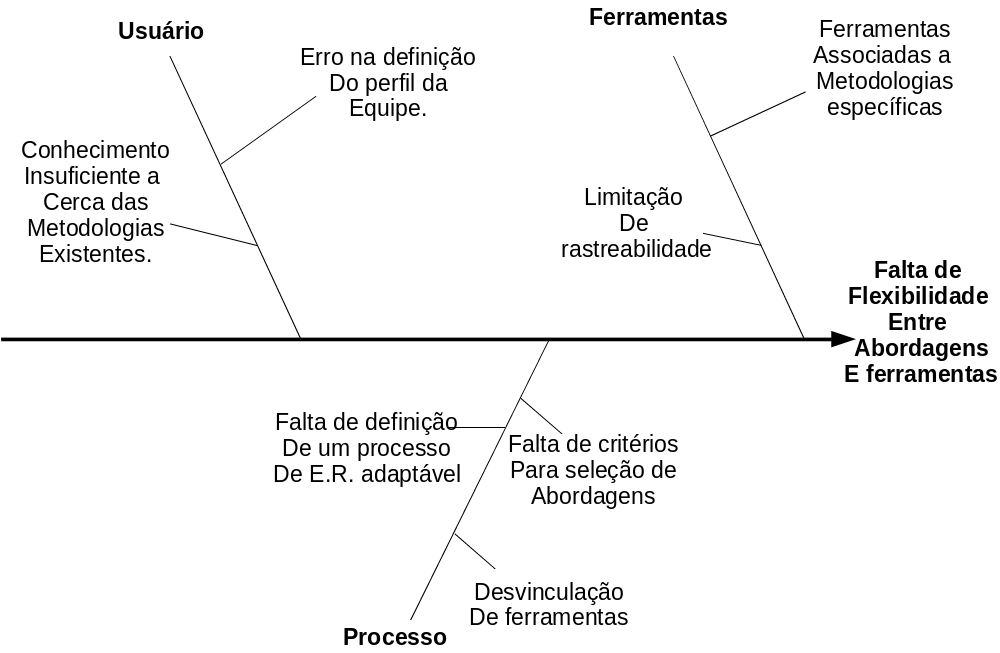
\includegraphics[width=0.8\textwidth]{imgModelagem/fishbone}
	\caption{Diagrama de Ishikawa}
	\label{img:fishbone}
\end{figure}
%-------------------------------------FISHBONE AQUI----------------------------------------


%-------------------------------------FRAMEWORK DE Problema-----------------------------------
Para melhor entendimento do problema, utilizamos a técnica de \textit{Framework de problema}, que consiste em criar uma tabela apresentando o problema, os afetados, o impacto e qual seria uma solução bem sucedida, o Framework esta retratado na tabela \ref{tab:frameworkproblema}.

\begin{table}[htbp]
\centering
\begin{tabular}{|p{3cm}|p{10cm}|p{2.5cm}|}
%----------------------------------------------
\hline
\textbf{O Problema:} &
Falta de flexibilidade entre Abordagens e Ferramentas. 
\\ \hline
%----------------------------------------------
\textbf{Afeta:} &
Todos os desenvolvedores de \sw~que necessitam de uma flexibilidade maior na gerência de requisitos.
\\ \hline
%----------------------------------------------
\textbf{Cujo impacto é:} &
Processo de requisitos mal gerenciados, aumentando a possibilidade de erros durante o desenvolvimento.
\\ \hline
%----------------------------------------------
\textbf{Uma solução bem sucedida seria:} &
Utilização de uma ferramenta que faça gerência de requisitos de forma flexivel, podendo utilizá-la em qualquer metodologia.
\\ \hline
%----------------------------------------------
\end{tabular}
\caption{Framework de Problema}
\label{tab:frameworkproblema}
\end{table}

%-----------------------------------------FRAMEWORK DE NECESSIDADES----------------------------------------
Após o entendimento do problema, vê-se necessária a documentação das necessidades do cliente. Utilizou-se de uma técnica chamada \textit{framework de necessidades} na qual são apresentados todos os problemas, as necessidades, a solução atual e a solução proposta. Dessa forma, pode-se obter um entendimento mais organizado dos problemas e necessidades do cliente, de acordo com o retradado na tabela \ref{tab:frameworknecessidade}.

\begin{table}[H]
\centering
\begin{tabular}{|p{5cm}|p{3cm}|p{3cm}|p{5cm}|}

%-------------------------------------------------------------
\hline
\textbf{Necessidade} &
\textbf{Problema} &
\textbf{Solução Atual} &
\textbf{Solução Proposta}
\\ \hline
%-------------------------------------------------------------
Utilização de ferramentas que se adequem as metodologias. &
Ferramentas associadas a metodologias específicas. &
Equipe utiliza mais de uma ferramenta para abranger as abordagens utilizadas. &
Criação de uma ferramenta que seja flexível para qualquer metodologia, abrangendo todas as agordagens e até a mesclagem das mesmas.
\\ \hline
%-------------------------------------------------------------
Apoio a utilização de uma rastreabilidade organizada e eficiente em qualquer abordagem. &
Limitação de ratreabilidade. &
A equipe precisa criar sua rastreabilidade sem o apoio de uma ferramenta flexível. &
Criação de uma ferramenta que gere a rastreabilidade dos requisitos de forma organizada e eficiente para qualquer abordagem.
\\ \hline
%-------------------------------------------------------------
Obter critérios fixos que redirecionem o projeto para a abordagem mais adequada. &
Falta de critérios para seleção de abordagens. &
Equipe precisa estudar as características do projeto e decidir qual a abordagem mais adequada. &
Criação de uma ferramenta que recolha as características do projeto e apresente a abordagem mais adequada.
\\ \hline
%-------------------------------------------------------------
Utilização de apenas uma ferramenta de gerência de requisitos durante o projeto. &
Desvinculação de Ferramentas. &
Equipe utiliza mais de uma ferramenta. &
Criação de uma ferramenta que garanta as funcionalidades de todas as ferramentas baseadas em distintas abordagens. 
\\ \hline
%-------------------------------------------------------------
Obter um processo de \textit{E.R.} adaptável a qualquer abordagem. &
Falta de definição de um processo de \textit{E.R.} adaptável. &
Utilização de um processo inflexível e voltado apenas para uma abordagem. &
Criação de uma ferramenta que gerencie processos flexíveis.
\\ \hline
%-------------------------------------------------------------
Obter o perfil da equipe de forma adequada. &
Erro na definição do perfil da equipe. &
Equipe precisa definir o próprio perfil. &
Criação de uma ferramenta que receba \textit{inputs} das características da equipe e apresente o perfil da equipe de forma correta.
%-------------------------------------------------------------
\\ \hline
Utilização da metodologia mais adequada para as características do projeto.&
Conhecimento insuficiente a cerca das metodologias existentes. &
Equipe precisa estudar todas as metodologias para escolher a mais adequada. &
Criação de uma ferramenta que apresente a metodologia mais adequada para o projeto.
\\ \hline
%-------------------------------------------------------------
\end{tabular}
\caption{Framework de Necessidades}
\label{tab:frameworknecessidade}
\end{table}

%-----------------------------------------------------------------------------------------------------------
\subsection{Visão Geral do Produto}
	
Nesta seção, pode-se ter um entendimento geral de como será o produto final, quais serão suas características, como serão suas funcionalidades e etc.

\subsubsection{Perspectiva do Produto}
	
O produto se encontrará em um contexto onde existem inúmeras ferramentas com o mesmo propósito, porém, as ferramentas existentes são inflexíveis quando se trata da abordagem que será seguida durante o desenvolvimento de \sw. Esta falha será corrigida na \nomeferramenta, que irá propor uma metodologia para cada projeto em particular de acordo com suas características.

A ferramenta pode ser autocontida, não necessitando do apoio de nenhum outro sistema, porém a utilização de ferramentas de modelagem de processos é bastante indicada para que a máxima organização do projeto seja alcançada.

\subsubsection{Resumo das Capacidades}
	
O grande diferencial da \nomeferramenta~ será a flexibilização na abordagem que será seguida durante o gerenciamento de projetos de \sw. O sistema deverá indicar a melhor abordagem a ser seguida pela equipe de desenvolvimento, garantindo a otimização do processo de desenvolvimento.

A ferramenta será capaz de disponibilizar a opção de modificar a abordagem indicada pela ferramenta, para que a equipe de desenvolvimento possa escolher a abordagem na qual os mesmos se sentem mais a vontade.

%-----------------------------------------------------------------------------------------------------------
\subsection{Recursos do Produto}

Os recursos do produto são as funcionalidades do sistema com uma pequena descrição, o que futuramente será transformado em casos de uso, e que serão detalhados no documento de casos de uso, presente na sessão \ref{sec:documento_de_caso_de_uso} deste documento, e estão listados a seguir.

\begin{enumerate}
	\item Definir Metodologia
	\item Manter Problema
	\item Manter Necessidades
	\item Manter Características
	\item Manter Casos de Uso
	\item Manter Temas de Investimento
	\item Manter Épicos
	\item Manter Features
	\item Manter Histórias de Usuário
	\item Manter Atributos
	\item Manter Rastreabilidade de Requisitos
	\item Gerar \textit{Diagrama de Ishikawa}
	\item Manter Atores do Projeto
	\item Gerar Diagramas de Casos de Uso
	\item Manter \textit{Roadmaps}
	\item Gerar plano de iteração
	\item Definir ``hibridez'' do projeto
	\item Controlar histórico de versão
\end{enumerate}
%-----------------------------------------------------------------------------------------------------------
\subsection{Restrições}
\subsubsection{Restrição Técnica}

A ferramenta poderá ser executada pelos navegadores Google Chrome versão 37.0.2062.120 ou superior Firefox versão 33.0 ou superior, não sendo possível sua utilização no Internet Explorer ou Safari.

%Observe todas as restrições de design, restrições externas, como requisitos operacionais ou regulamentares) ou outras dependências.

%-----------------------------------------------------------------------------------------------------------
\subsection{Faixas de Qualidade}
%Defina as faixas de qualidade para desempenho, robustez, tolerância a falhas, usabilidade e características similares que o conjunto de recursos não descreve.

%-----------------------------------------------------------------------------------------------------------

\subsection{Atributos do Recurso}

Atributos de recursos são basicamente descrições dos requisitos em alguma área em específico. Durante o projeto foram utilizados os atributos de arquitetura, prioridade e status.

\subsubsection{Atributos de Arquitetura\\}

Atributos de arquitetura são atributos que definem a complexidade arquitetural de se implementar algum requisito, por exemplo, se haverá necessidade de alterar arquitetura do software, e estão retratados na tabela \ref{tab:atributo_arquitetura}

\begin{table}[H]
\begin{tabular}{|p{4cm}|p{11cm}|}
%-------------------------------------------
\hline
\textbf{Atributo} &
\textbf{Descrição}
\\ \hline

%-------------------------------------------
\textbf{Grande} &
Para implementar o requisito, a arquitetura sofrerá uma grande alteração
\\ \hline

%-------------------------------------------
\textbf{Média} &
A arquitetura terá uma alteração consideravel na implementação do requisito
\\ \hline

%-------------------------------------------
\textbf{Baixa} &
A arquitetura terá uma pequena alteração para sustentar o requisito
\\ \hline

%-------------------------------------------
\textbf{Nenhuma} &
O requisito não terá impacto nenhum na arquitetura do projeto
\\ \hline
\end{tabular}
\caption{Atributo de Arquitetura}
\label{tab:atributo_arquitetura}
\end{table}

\subsubsection{Atributo de Prioridade\\}

Atributos de prioridade são atributos que definem o quão importante um requisito é para o cliente, definindo se ele deve ser implementado o mais rápido possível ou se pode ter sua implementação adiada, estão retratados na tabela \ref{tab:atributo_prioridade}.

\begin{table}[H]
\begin{tabular}{|p{4cm}|p{11cm}|}

\hline
\textbf{Atributo} &
\textbf{Descrição}
\\ \hline

%-----------------------------------------
\textbf{Alta prioridade} &
Os requisitos marcados com este atributo são requisitos que possuem um grande interesse do cliente
\\ \hline

%-----------------------------------------
\textbf{Média prioridade} &
Os requisitos marcados por este atributo são requisitos que o cliente possui um grande interesse, porém não existe necessidade de implementá-lo rapidamente.
\\ \hline

%----------------------------------------
\textbf{Baixa prioridade} &
Os requisitos marcados por este atributo são requisitos que o cliente deseja, porém não são essenciais para o funcionamento da solução.
\\ \hline

\end{tabular}
\caption{Atributo de prioridade}
\label{tab:atributo_prioridade}
\end{table}

\subsubsection{Atributos de Status\\}

Atributos de status são atributos que indicam em que fase um requisito está, de acordo com a tabela a seguir, e estão retrados na tabela \ref{tab:atributo_status}

\begin{table}[h]
\begin{tabular}{|p{4cm}|p{11cm}|}

\hline
\textbf{Atributo} &
\textbf{Descrição}
\\ \hline

%-------------------------------
\textbf{Aceito} &
Requisito devidamente implementado e aceito pelo cliente
\\ \hline

%-------------------------------
\textbf{Implementado} &
Requisito implementado porém esperando aceitação
\\ \hline

%-------------------------------
\textbf{Detalhado} &
Requisito detalhado, esperando por implementação
\\ \hline

%------------------------------
\textbf{Elicitação aceita} &
Requisito elicitado e aceito pelo cliente porém sem detalhamento
\\ \hline

%------------------------------
\textbf{Elicitado} &
Elicitado porém esperando aceitação do cliente
\\ \hline

\end{tabular}
\caption{Atributo de status}
\label{tab:atributo_status}
\end{table}